% Copyright (C) 2019 BARBOTIN Nicolas
\documentclass[a4paper,12pt]{article}

\usepackage[french]{babel}
\usepackage[T1]{fontenc}
\usepackage[utf8]{inputenc}
\usepackage[sfdefault]{roboto}
\usepackage{courier}
\usepackage{fullpage}
\usepackage{fancyhdr}
\usepackage{lastpage}
\usepackage{xcolor}
\usepackage{float}
\usepackage{titling}
\usepackage{tikz}
\usepackage{listings}
\usepackage{glslListings}
\usepackage{calc}
\usepackage[compact]{titlesec}
\usepackage{graphicx} %\usepackage{subfig} %%Subfigures inside a figure
%\usepackage{setspace}

%% Math Packages
\usepackage{amsmath}
\usepackage{amsthm}
\usepackage{amsfonts}
\usepackage{stmaryrd}

%% Document properties
\title{IN55 -- Rapport de projet}
\author{A. Einholtz et N. Barbotin}

%% PDF Meta
\usepackage[pdftex,
            pdfauthor={\theauthor},
            pdftitle={\thetitle}]{hyperref}

%% Line Spacing
%\singlespacing        %% 1-spacing (default)
%\onehalfspacing       %% 1,5-spacing
%\doublespacing        %% 2-spacing

%% Custom Colors
\definecolor{dgray}{gray}{0.25}
\definecolor{dgreen}{rgb}{0,0.5,0}
\definecolor{preprocessor}{rgb}{0.5,0.25,0}
\definecolor{glslType}{rgb}{0.5,0,1}


%% Page style
\pagestyle{fancy}
\renewcommand{\headrulewidth}{0pt}
\fancyhead{}
\fancyfoot[L]{\fontsize{11pt}{11pt}\selectfont\textcolor{dgray}{\theauthor}}
\fancyfoot[C]{} %\fancyfoot[C]{\fontsize{11pt}{11pt}\selectfont\textcolor{dgray}{\thetitle}} % Broken by titlesec ?!
\fancyfoot[R]{\fontsize{11pt}{11pt}\selectfont\textcolor{dgray}{Page \thepage\ sur \pageref*{LastPage}}}

%% Custom Math Operators
\DeclareMathOperator{\sinc}{sinc}

%% Custom commands
\newcommand*\circled[1]{\tikz[baseline=(char.base)]{
            \node[shape=circle,draw,inner sep=0.25pt] (char)
            {\rule[-3pt]{0pt}{\dimexpr2ex}#1};}}

\newcommand{\svg}[2][0cm]{
    \begin{figure}[H]
        \centering
        \def\svgwidth{\columnwidth - #1}
        \input{#2.pdf_tex}
    \end{figure}
}

\newcommand{\shadersrc}[1]{
    \lstinputlisting[language=GLSL]{../shaders/#1}
}

\newcommand{\abs}[1]{\left\lvert #1 \right\rvert}

%% Language styles
\lstset{language=GLSL,
        basicstyle=\ttfamily,
        keywordstyle=[1]\color{glslType}\ttfamily,
        keywordstyle=[2]\color{blue}\ttfamily,
        keywordstyle=[3]\color{blue}\ttfamily,
        keywordstyle=[4]\color{preprocessor}\ttfamily,
        stringstyle=\color{red}\ttfamily,
        commentstyle=\color{dgreen}\ttfamily,
        showstringspaces=false,
        frame=single,
        rulecolor=\color{gray},
        aboveskip=8pt,
        belowskip=0pt,
        breaklines=true,
        postbreak=\mbox{\textcolor{red}{$\hookrightarrow$}\space}
}

%%%%%%%%%%%%%%%%%%%%%%%%%%%%%%%%%%%%%%%%%%%%%%%%%%%%%%%%%%%%%%%%%%%%%%%%%%%%%%%%%%%%%%%%%%%%%%%%%%%%%%%%%%%%%%%%%%%%%%%%%%
%% DOCUMENT
\begin{document}
\setlength{\parindent}{0cm}
\setlength{\parskip}{8pt}

\begin{center}
    % Title
    \Huge\thetitle

    \vfill
    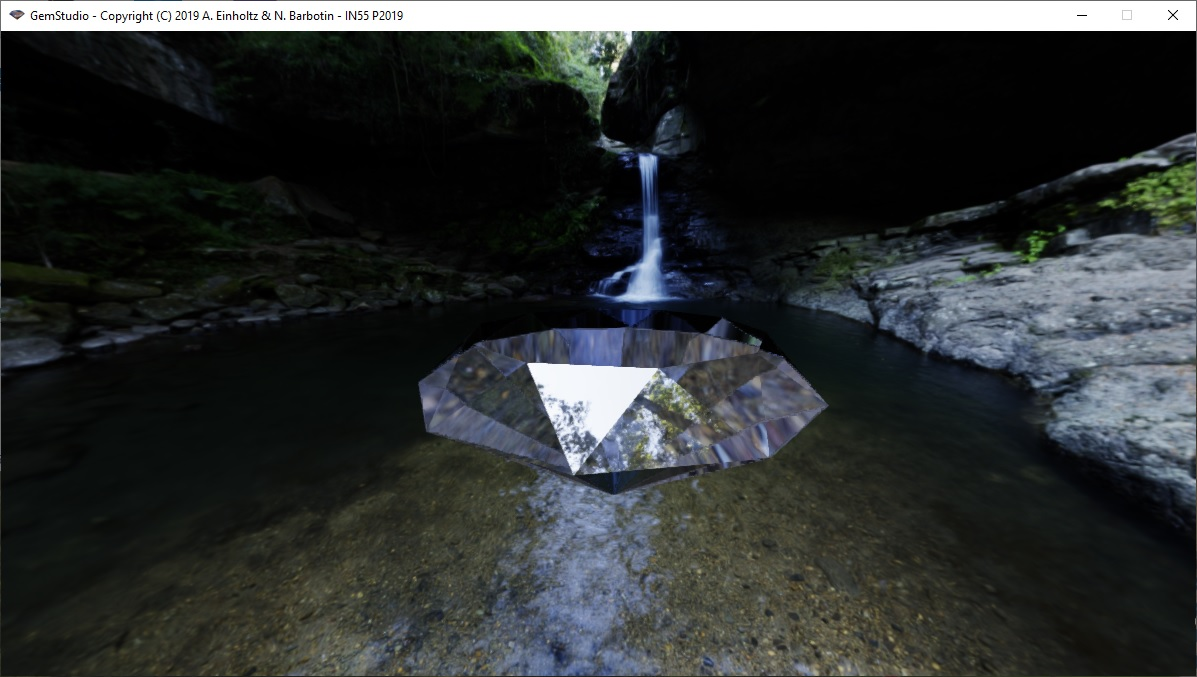
\includegraphics[width=15cm]{screenshot.jpg}
    \vfill
\end{center}

\newpage
\tableofcontents

\newpage
\part{Introduction}
\section{Présentation du projet}
Dans le cadre de l'UV IN55 lors du semestre de printemps 2019, nous avons été chargé de réaliser
un projet basé sur OpenGL. Le sujet que nous avons sélectionné visait à faire le rendu de pierres
précieuses en temps réel. Pour cela, nous avons utilisé C++ avec les bibliothèques GLFW pour la
gestion de la fenêtre et GLEW pour le chargement d'OpenGL. Les mathématiques et l'interface graphique
sont gérées par des bibliothèques maisons, soit MGPCL et AISO.

\section{Utilisation}
TODO: décrire comment utiliser le projet (contrôle caméra etc...)

\section{Distribution des tâches}
osef

\section{Choix techniques}
Deux effets principaux interviennent dans le visuel des pierres précieuses: la réflection et la réfraction.
Ces effets étant difficile à mettre en œuvre en temps réel (c'est-à-dire, sans raytracing), nous avons décidé
de se limiter à un seul et unique objet dans toute la scène: la pierre précieuse. Celle-ci est placée dans un
décor reposant sur une \emph{environment map}; il s'agît d'une texture qui considérée comme \og à l'infini \fg
\ par rapport à la caméra. Cela permet d'accélérer de manière importante le rendu et permet d'atteindre une
centaine d'images par seconde sur une Intel HD Graphics 620, toute en gardant une qualité décente.

En plus de la réflection et de la réfraction, nous avons décidé d'implémenter les effets suivants:
\begin{itemize}
    \item Pipeline \emph{High-Dynamic Range} (HDR), pour assurer la qualité des réflections
    \item Exposition automatique: contrôle automatiquement la luminosité de la scène de manière à percevoir un maximum de couleurs différentes
    \item Bloom: effet d'éblouissement lorsque la caméra est exposée à une lumière importante
    \item Lens flare: imitation des artéfacts visuels produit par les imperfections des lentilles, perçus généralement lorsque le soleil fait directement face à la caméra
    \item Fast Approximative Anti-aliasing (FXAA) pour réduire \og l'aliasing \fg
\end{itemize}

\part{Fonctionnement}
\section{Fonctionnement général}
Les diagrammes UML iront ici, décrire aussi comment la forme de la gemme est générée

\section{Pipeline de rendu}
Le rendu de la scène est réalisé avec la pipeline suivante:
\svg{PipelineDeRendu}

\section{Passe de rendu principale}
La passe de rendu principale est celle durant laquelle les éléments visuels principaux sont dessinés; c'est-à-dire
la \emph{skybox} et la gemme. Comme il s'agît d'une passe de rendu HDR, cette passe de rendu prends en compte
l'exposition déterminée par le système d'exposition automatique, décrit plus bas. Enfin, cette passe de rendu
génère en plus du color buffer habituel, un second buffer HDR qui sera plus tard utilisé pour le \emph{bloom}
(l'effet d'éblouissement). Ce buffer est princialement noir, sauf aux endroits où la couleur dépasse un
seuil de luminance définit par l'utilisateur. Dans ce cas, le buffer de bloom contient la même valeur que le color
buffer. Ceci se résume par le code GLSL suivant:

\begin{lstlisting}
float luma = dot(final, vec3(0.2126, 0.7152, 0.0722));

if(luma > u_BloomThreshold)
    out_Bloom = vec4(final, 1.0);
else
    out_Bloom = vec4(vec3(0.0), 1.0);
\end{lstlisting}

La \emph{skybox} est un simple cube texturé avec l'\emph{environment map} décrite plus haut. Normalement, les faces
de la skybox doivent être placées à une distance infinie de la caméra. Comme nous ne pouvons pas vraiment faire cela,
nous simulons cet effet en placant le centre du cube à la position de la caméra, et en désactivant l'écriture dans le buffer
de profondeur (\emph{glDepthMask}). Ainsi, tout objet déssiné après la skybox, qu'il soit devant ou derrière
celle-ci, sera tout de même déssiné à l'écran. Puisque c'est elle qui émet la lumière de toute la scène, le dessin de
ce cube est fait sans aucun calcul d'illumination.

La gemme, en revanche, subit quelques calculs d'illumination. Les deux effets à prendre en compte sont (comme dit
précédemment) la réflexion et la réfraction.

\end{document}
